\begin{figure*}[t]
  \centering
  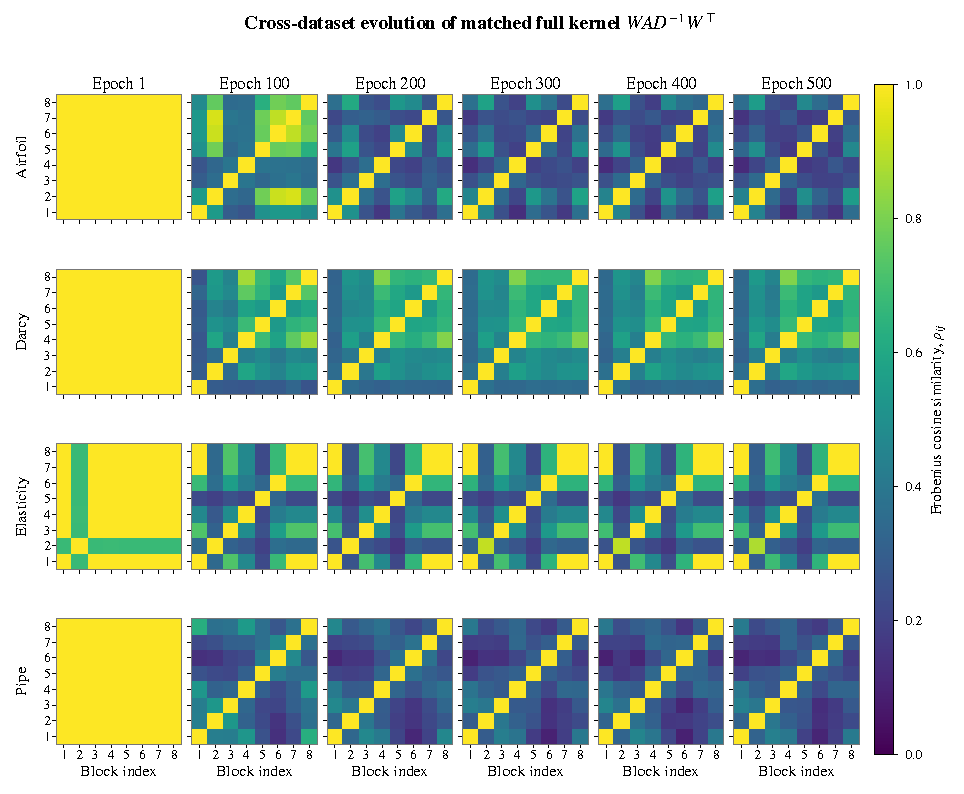
\includegraphics[width=\linewidth]{four_dataset_full_kernel_heatmaps.pdf}
  \caption{\textbf{Evolution of cross-layer propagation-kernel similarity across four PDE benchmarks.}
  Rows correspond to Airfoil, Darcy, Elasticity, and Pipe; columns show epoch 1,
  followed by epochs 100, 200, 300, 400, and 500. Each cell is the
  sample-mean Frobenius cosine similarity between two blocks, after optimal head matching.
  The displayed full propagation kernel is $P^{\mathrm{full}}=WAD^{-1}W^\top$ and all panels use
  one common 0--1 color scale. The epoch-1 panel is sourced from the monitor's validation\_000001
  snapshot, recorded after the first training epoch.}
  \label{fig:four-dataset-full-kernel-heatmaps}
\end{figure*}
